The introduction section serves as the opening chapter of this internship report, providing an insightful overview of the internship experience, its significance, and the structure of the subsequent report. This section sets the context by introducing the organization where the internship took place, presenting the objectives pursued, highlighting the relevance of the internship experience, and offering a glimpse into the report's content.

\section{Background}

In the backdrop of an ever-evolving global landscape, industries are undergoing rapid transformations driven by technological advancements and shifting consumer behaviors. Within this dynamic environment, the opportunity to engage in a hands-on internship plays a crucial role in bridging the gap between theoretical knowledge and practical application.

This internship occurred within the dynamic realm of electronics, networking, and computer building. The host organization, NetLab!UG, stands as a prominent player within this industry, renowned for its commitment to deploying solutions that leverage research cores to address the needs of both national and international development, in alignment with the Sustainable Development Goals (SDGs).
\subsection{Objectives}

The primary objectives of this internship were thoughtfully formulated to align with both personal and professional growth aspirations. With a keen desire to consolidate classroom learning into real-world scenarios, the goals included:
\begin{enumerate}
    \item.\textbf{Hands-On Experience in Desktop Computer Building:} To acquire practical skills in assembling and configuring desktop computer systems, gaining a deep understanding of hardware components and their interactions.

    \item.\textbf{Server Administration Proficiency:} To develop expertise in server administration, including tasks such as server setup, maintenance, security, and troubleshooting.

    \item.\textbf{Networking Competence:} To enhance networking knowledge and skills, with a focus on designing, configuring, and managing network infrastructure.

    \item.\textbf{Manufacturing Insights:} To gain insights into the manufacturing processes, quality control, and production workflows related to electronics and computer hardware.
\end{enumerate}
By engaging with these objectives, the intention was not only to contribute to the organization's initiatives but also to enhance individual capabilities across desktop computer building, server administration, networking, and manufacturing.

\subsection{Internship Location}

The internship was primarily conducted at two distinct locations, each serving a specific purpose:

\textbf{Makerere University Netlabs Ewaste Lab:} This facility served as the central hub for the internship, housing the computers and being the primary location for software-related tasks. It provided an ideal environment for hands-on experience with computer hardware and software configurations.

\textbf{GNEX, Supported by Motiv Uganda:} For manufacturing-related activities, the equipment and resources were made available at Motiv Uganda, with support from GNEX. This partnership allowed for the design and production of computer cases and hardware components. It provided valuable insights into the manufacturing processes associated with electronics and computer hardware.

\section{Company Profile}

\subsection{Introduction}

NetLabs!UG is a Research Centre of Excellence (CoE) specializing in telecommunications and networking technologies. In an era marked by technological transformation, including the Internet of Things (IoT) and Artificial Intelligence (AI), NetLabs!UG plays a pivotal role in supporting academic development and facilitating commercial interests within Uganda and East Africa.

\subsection{Innovation and Research}

Innovation is at the core of NetLabs!UG's research activities. As a CoE, innovation is a fundamental element of their research process. Their commitment to innovation aligns with the evolving technology landscape, and they emphasize its importance alongside traditional research pursuits. This two-strand approach positions Uganda and East Africa as hubs for development and innovation in this critical sector.

\subsection{Vision of netLabs!UG}
To be regional leader in collaborative research, development and solutions on innovative telecommunication and networking technologies, strengthening the Ugandan
and Regional technologies economy.

\subsection{Mission of netLabs!UG}
To be a regional Centre of Excellence in the area of telecommunications and networking technologies, ensuring an independent source of advice for government
policy as well as an independent source of research, development and solutions support to telecommunication companies and enterprises in Uganda and the region of
East Africa.

\subsection{NetLabs Logo}

\begin{figure}[H]
    \centering
    
\includegraphics{images/netlabs-logo.png}
    \caption{NetLabs Logo}
\end{figure}


\section{Company Structure}

\begin{figure}[H]
    \centering
    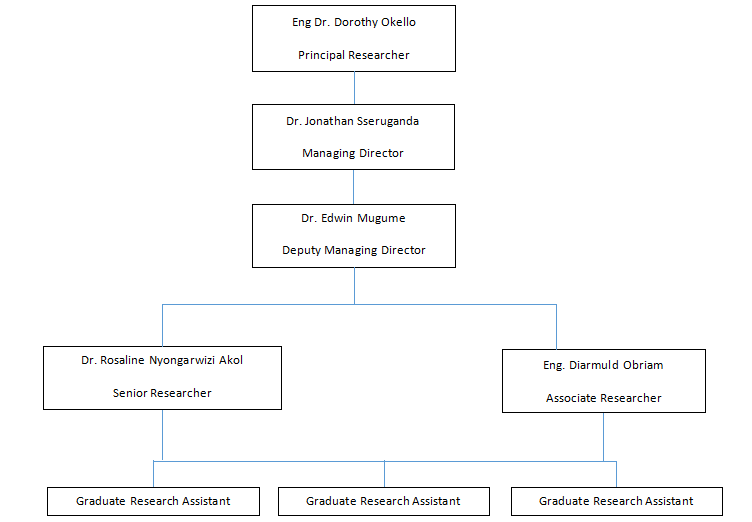
\includegraphics{images/netlabs-struct.png}
    \caption{NetLabs Organisational Structure}
    \label{fig:netlabs-struct}
\end{figure}

Figure \ref{fig:netlabs-struct} shows the hierarchical arrangement of the lines of authority, communication, rights and duties of netLabs!UG. It determines how roles, power and responsibilities are assigned, controlled and how information flows between the different
levels of management.

\section{Objectives of netLabs!UG}
\begin{enumerate}
    \item To engage in industry partnership with vendors and other Research and Development centres and carriers.
    \item To support the incubation of innovation ideas.
    \item To build technical intelligence.
    \item To support undergraduate industrial training to identify and nurture talent.
    \item To support high technology Foreign Direct Investment Companies.
    \item To engage in industry
\end{enumerate}

Understanding the roles and responsibilities of key personnel and the structure of functional divisions within netLabs!UG will provide valuable context for the experiences and insights gained during the internship.

\section{Relevance of Internship}

The internship experience at NetLabs!UG holds profound relevance within the broader context of my academic and career aspirations. This section delves into the specific aspects of the internship that make it highly pertinent and valuable.

\subsection{Alignment with Academic Studies}

The internship was meticulously chosen to align with my academic pursuits as an Electrical Engineering student at Makerere University. The practical exposure gained during this internship complements the theoretical foundation provided by my coursework. It allowed me to apply classroom knowledge to real-world scenarios, bridging the gap between theory and practice.

\subsection{Hands-On Learning}

One of the key facets that underline the relevance of this internship is the opportunity for hands-on learning. Engaging in PC building provided me with invaluable experiences that textbooks and lectures alone cannot offer. These hands-on experiences enhanced my problem-solving skills, critical thinking abilities, and technical proficiency.

\subsection{Industry Relevance}

The internship took place within the dynamic realm of [product development, a field that is witnessing rapid technological advancements and innovation. By immersing myself in this industry, I gained insights into the latest trends, emerging technologies, and best practices. This industry relevance is instrumental in preparing me for a successful career in the ever changing Electrical Engineering.

\subsection{Professional Growth}

Beyond academic relevance, the internship significantly contributed to my professional growth. Working alongside experienced professionals at Gnex and NetLabs exposed me to industry-standard practices and protocols. The mentorship and guidance received from Dr Edwin Mugume played a pivotal role in shaping my understanding of the field.

\subsection{Networking Opportunities}

During the internship, I had the privilege of networking with professionals, experts, and peers in the industry. These connections have the potential to open doors to future opportunities, collaborations, and career prospects. The relationships forged during this internship are invaluable assets.

In summary, this internship holds immense relevance by aligning with my academic studies, offering hands-on learning experiences, providing industry exposure, fostering professional growth, and creating networking opportunities. These aspects collectively enrich my academic journey and prepare me for a successful career.
\section{Scope}

The scope of this internship report encompasses a comprehensive overview of the experiences, activities, and insights garnered during the internship. From engaging in hands-on tasks  to collaborating with cross-functional teams and departments, the scope of this report extends to the intricacies of practical application and the broader understanding.

Specifically, this report will cover:
\begin{enumerate}
    \item \textbf{Hands-On Tasks:} A detailed account of the practical tasks and projects I was involved in during the internship, including [list specific tasks or projects].
    \item \textbf{Cross-Functional Collaboration:} Insights into my collaboration with various teams and departments within NetLabs!UG and GNEX, highlighting the interdisciplinary nature of the internship.
    \item \textbf{Applied Knowledge:} The practical application of academic knowledge and theoretical concepts to real-world scenarios, providing examples and outcomes.
    \item \textbf{Challenges and Solutions:} An analysis of challenges encountered during the internship and the strategies employed to overcome them.
    \item \textbf{Learning and Growth:} Reflections on personal and professional growth, skill development, and the acquisition of industry-specific knowledge.
    \item \textbf{Relevance to Career Goals:} An exploration of how the internship experience aligns with my long-term career aspirations and the valuable insights gained for future endeavors.
\end{enumerate}
This report aims to provide a comprehensive narrative of the internship journey, from day-to-day tasks to overarching insights, contributing to a holistic understanding of the practical application of Electrical Engineering concepts within the dynamic environment of NetLabs!UG.

\section{Structure of the Report}

The subsequent sections of this report are structured to delve into the various dimensions of the internship journey.

\textbf{Chapter 1: Introduction}

In this chapter, I provide an insightful overview of the internship experience, its significance, and the structure of the subsequent report. I introduce the organization where the internship took place, present the objectives pursued, highlight the relevance of the internship experience, and offer a glimpse into the report's content.

\textbf{Chapter 2: Literature Review}

Chapter [2] delves into a comprehensive review of the relevant literature and theoretical concepts related to the field of Electrical Engineering. It sets the theoretical foundation for understanding the practical aspects discussed in later chapters.

\textbf{Chapter 3: Work Done}

Chapter [3] provides a detailed account of the tasks, projects, and responsibilities undertaken during the internship. I discuss the challenges encountered, innovative solutions devised, and practical experiences gained.

\textbf{Chapter 4: Conclusions}

In the final chapter, I draw conclusions based on the internship experiences and reflect on the overall impact of this journey on my personal and professional growth. I also discuss the relevance of the internship to my academic and career goals, and provide recommendations or insights for future interns.

This structured report aims to provide a comprehensive and informative account of my internship experience, from the theoretical foundations to the practical application and concluding reflections.
